
\documentclass{aa}  

%
\usepackage{graphicx}
\usepackage[table]{xcolor}
%%%%%%%%%%%%%%%%%%%%%%%%%%%%%%%%%%%%%%%%
\usepackage{txfonts}
\usepackage{bm}
\usepackage{multirow, makecell}
\usepackage{booktabs}
%%%%%%%%%%%%%%%%%%%%%%%%%%%%%%%%%%%%%%%%

\usepackage[colorlinks=true,citecolor=blue,linkcolor=blue,urlcolor=blue]{hyperref}
\begin{document} 

\title{Likelihood Implicit Methods}


\newcommand{\justine}[1]{{\color{cyan}JZ: #1}}
\newcommand{\denise}[1]{{\color{red}DL: #1}}
\newcommand{\FL}[1]{{\color{magenta}FL: #1}}
\newcommand{\LM}[1]{{\color{olive}LM: #1}}

\author{Denise Lanzieri \inst{1}
\and
Justine Zeghal \inst{2}
\and
T. Lucas Makinen \inst{3}
\and
Alexandre Boucaud \inst{2}
\and
Fran\c{c}ois Lanusse \inst{4}
\and
Jean-Luc Starck \inst{4}
}
\institute{Université Paris Cité, Université Paris-Saclay, CEA, CNRS, AIM, F-91191, Gif-sur-Yvette, France
\and
Université Paris Cité, CNRS, Astroparticule et Cosmologie, F-75013 Paris, France
\and Imperial Centre for Inference and Cosmology (ICIC) $\&$ Astrophysics Group, Imperial College London, Blackett Laboratory, Prince Consort Road, London SW7 2AZ, United Kingdom
\and
Université Paris-Saclay, Université Paris Cité, CEA, CNRS, AIM, 91191, Gif-sur-Yvette, France
}
\titlerunning{}
\date{Received xxx; accepted xxx}


 
  \abstract
  % context heading (optional)
  % {} leave it empty if necessary  
   {blabla}
  % aims heading (mandatory)
    {blabla}
  % methods heading (mandatory)
    {blabla}
  % results heading (mandatory)
   {blabla}
  % conclusions heading (optional), leave it empty if necessary 
   {}

   \keywords{methods: statistical – gravitational lensing: weak – cosmology: large-scale structure of Universe
               }
               

   \maketitle

%-------------------------------------------------------------------
%------------------------------------------------------------------
%------------------------------------------------------------------
%------------------------------------------------------------------
\section{Introduction}
Weak gravitational lensing by the large-scale structure is caused by the presence of foreground matter bending the light emitted by background galaxies. Being sensitive to the large-scale structure of the universe, it is one of the most promising tools for investigating the nature of dark energy, the origin of the accelerating expansion of the universe and estimating cosmological parameters. Future cosmological surveys, such as the Legacy Survey of Space and Time (LSST) of the Vera C. Rubin Observatory \citep{ivezic2019lsst}, the Nancy Grace Roman Space Telescope \citep{spergel2015wide}, and  the Euclid Mission \citep{laureijs2011euclid}, will rely on weak gravitational lensing as one of the principal physical probes to address unresolved questions in current cosmology.
 As these surveys become deeper, they will be able to access more non-Gaussian features of the matter fields. This makes the standard weak lensing analyses, which rely on two-point statistics such as the 2-point shear correlation or the angular power spectrum, sub-optimal. These analyses are unable to fully capture the non-Gaussian information imprinted in the lensing signal and can only access Gaussian information.


To overcome this limitation, several higher-order statistics have been introduced. These include weak lensing peak counts \citep{liu2015cosmology,  liu2015cosmological, lin2015new, kacprzak2016cosmology, peel2017cosmological, shan2018kids, martinet2018kids, ajani2020constraining, harnois2021cosmic, zurcher2022dark}, wavelet and scattering transform \citep{ajani2021starlet, cheng2021weak}, the one point PDF \citep{liu2019constraining, uhlemann2020fisher, boyle2021nuw}, Minkowski functionals \citep{kratochvil2012probing, petri2013cosmology}, moments of mass maps \citep{gatti2021dark},  and 3 point statistics \citep{takada2004cosmological, semboloni2011weak, rizzato2019tomographic, halder2021integrated}. 
Although these methods have proven to improve cosmological constraints, they rely on summary statistics, for which an analytical description is often lacking. These methods frequently assume a Gaussian likelihood and require accurate computation of the covariance matrix, which can be challenging.



One way to overcome the use of summary statistics and bypass the associated issues, such as the use of simplified and unjustified likelihood assumptions, is through the use of map-based approaches.
Within this category, a further distinction can be made between methods that integrate observations into a forward model allowing the exact reconstruction of the likelihood, and those designed to directly reconstruct the likelihood from synthetic data as part of the inference pipeline.
The former scenario, often referred to as Bayesian forward-modeling,  has gained popularity in the literature in the last decades \citep{schneider2015hierarchical, alsing2016hierarchical, alsing2017cosmological, bohm2017bayesian, porqueres2021bayesian, porqueres2022lifting, porqueres2023field}. Despite the differences among these works in terms of the physical models they assume or the specific quantities they aim to sample, they all demonstrate that conducting a field-level analysis results in more precise and accurate constraints compared to the two-point function analysis.
Despite the immense potential of these approaches, there is a noteworthy limitation: they frequently result in high-dimensional problems, necessitating the use of sophisticated statistical sampling techniques. \\
An alternative framework for inference is provided by Likelihood-Free Inference (LFI) approaches, which are sometimes referred to as Likelihood implicit or Simulation-Based Inference (SBI). \denise{TODO: cite some other work(?)}
The potential of LFI methods lies in the fact that they primarily rely on our ability to forward-simulate synthetic data, without the need for an explicit likelihood function. As a result, these methods are free from assumptions and approximations. Furthermore, incorporating systematic effects and complex physical processes into forward simulations is more straightforward compared to including them when constructing the likelihood function.
Given the potential of LFI methods, it is crucial to identify possible sources of bias and the associated challenges, as well as establish well-defined procedures to validate the results. For instance, it is widely recognized that even the most advanced LFI methods can be affected by the curse of dimensionality. This necessitates compression procedures that reduce the high-dimensional data set into a small number of summary statistics.
A significant question is how to design data compression procedures, aiming to derive low-dimensional summary statistics while minimizing information loss.



In this paper, we present a comparison of the performance of various neural network-based compression schemes within the Likelihood-Free Inference (LFI) framework. These methods differ in terms of the loss functions used to train the neural network, but they share the same inference strategy based on neural density estimation. Moreover, a crucial point is to validate the results obtained in the LFI context. To address this, we employ a Bayesian forward modeling approach that enables inference on the joint posterior of the cosmological parameters and the convergence field. The forward model is based on \texttt{SbiLens}, a Python package designed for Weak Lensing Implicit Inference with Differentiable Simulator implemented in \texttt{Jax}. \texttt{SbiLens} allows the sampling of convergence maps in a tomographic setting, accounting for the cross-correlation between different redshift bins.



The paper is structured as follows: in \autoref{Sec:Motivation}, we illustrate the motivation behind this work. In \autoref{Sec:the SBILens framework}, we introduce the \texttt{SbiLens} framework and describe the simulated data used in this work. In \autoref{Sec:experiment}, we detail the inference strategy and the three different approaches we used: the power spectrum, the map-based inference based on the Bayesian forward-modeling, and the map-based inference based on the LFI. In the same section, we also provide a detailed overview of different neural compression strategies. In \autoref{Sec:results}, we discuss the results and validate the LFI approaches. Finally, we conclude in \autoref{Sec:conclusion}. 







%------------------------------------------------------------------
%------------------------------------------------------------------
%------------------------------------------------------------------
%------------------------------------------------------------------
\section{Motivation}\label{Sec:Motivation}
%--------------------------------------------------------------------
With the increased statistical power of stage IV surveys, our cosmological analysis should not rely on the measurement of sub-optimal summary statistics, that may not fully capture the non-Gaussian information present in the lensing field at the scales accessible to future surveys. One of the main objectives of this paper is to introduce a forward model that directly extracts information from the raw pixel data, rather than relying on the analytical evaluation of summary statistics. By doing so, we aim to preserve all available information and facilitate the incorporation of systematic effects and the combination of multiple cosmological probes through joint simulations.
In this context, the simulator of the observables serves as our physical model, where each component is tractable. These models, also knows as \textit{probabilistic program}, considering a prior distribution $p(\bm{\theta})$ for the parameter $\bm{\theta}$, sample \textit{latent variables} $z_i \sim p_i(z_i|\bm \theta, z_{<i})$, generating the output $\bm x \sim p(\bm d|\bm \theta)$, where $\bm{d}$ represents the observations. However, computing the marginal likelihood is typically intractable:
\begin{equation}
    p(\bm{x}|\bm{\theta})=\int p(\bm{x},\bm{z}|\bm{\theta}) d\bm{z}=\int p(\bm{x}|\bm{z},\bm{\theta})p(\bm{z}|\bm{\theta}) d\bm{z}.
\end{equation}
To overcome this limitation while still capturing the full information content of the data, different approaches have been proposed in the literature. Although these approaches are often referred to by different names, in this work, we will make the following distinction
%--------------------------------------------------------------------
\paragraph{\textbf{Explicit inference}} referring to all Likelihood-based inference approaches. 
In the context of the forward model and full field analysis, fall in this category the Bayesian Hierarchical Model (BHM).
As a Bayesian forward approach it involves using a given model to predict observations and then comparing these predictions with real observations to infer the parameters of the model. The \textit{hierarchical} nature of this methodology comes from the fact that a complex inference task, such as the weak lensing inference task, can be broken down into several hierarchies of elements, which can be understood and from which we can sample from \citep{heavens2018bayesian}. However, performing a global analysis on complex and large datasets, such as what could be a lensing dataset, is not feasible. Therefore, the idea of dividing the global analysis into several subgroups, analyzing them in multiple steps, and using the output of each of those as input for the next one.  
This approach involves treating the simulator as a probabilistic model and performing inference over the joint posterior:
\begin{equation}
        p(\bm{\theta},\bm{z}|\bm{x})\propto  p(\bm{x},\bm{z}|\bm{\theta}) p(\bm{z}|\bm{\theta}).
\end{equation}
%--------------------------------------------------------------------
\paragraph{\textbf{Implicit inference}} referring to all the approaches not relying on an analytical model to describe the signal, but rather on learning the likelihood from simulations. This second class of approaches involves treating the simulator as a black box with only the ability to sample from the joint distribution
\begin{equation}
    (\bm{x}, \bm{\theta})\sim p(\bm{x}, \bm{\theta}).
\end{equation}
Within this class of methods, we can distinguish between more traditional methods such as the Approximate Bayesian Computation (ABC), a rejection-criteria based approach, which approximate the likelihood comparing the simulations with data, and the Density Estimation Likelihood Free Inference (DELFI), methods, where the inference task is approached as a density estimation problem.
Ultimately, for a given simulation model, the two approaches should converge to the same posterior.
%------------------------------------------------------------------
%------------------------------------------------------------------
%------------------------------------------------------------------
%------------------------------------------------------------------
\section{The SBILens framework}\label{Sec:the SBILens framework}
\subsection{Lognormal Modeling}
For various cosmological applications, the non-Gaussian field can be modeled as a Lognormal field \citep{coles1991lognormal,bohm2017bayesian}.
This model offers the advantage of generating the matter or convergence field rapidly while allowing the extraction of information beyond the two-point statistics. 
Although studies demonstrated that this model fails in describing the 3D field \citep{klypin2018density}, it properly describes the 2D convergence field \citep{clerkin2017testing, xavier2016improving}.
Assuming a simulated Gaussian convergence map $\kappa_g$, whose statistical properties are fully described by its power spectrum $C_{\ell}$ we know that this model is not a suitable representation of late-time and more evolved structures. One potential solution is to find a transformation $f(\kappa_g)$ of this map that captures the non-Gaussian features in the convergence field. In doing so, it is crucial to ensure that the transformed map maintains the correct mean and variance, effectively recovering the correct two-point statistics.
Denoting $\mu$ and $\sigma_g^2$ the mean and covariance matrix of $\kappa_g$ respectively, we can define the transformed convergence $\kappa_{ln}$ as a shifted lognormal random field:
\begin{equation}\label{Eq:log_norm_kappa}
    \kappa_{ln}=e^{\kappa_{g}}-\lambda, 
\end{equation}
where $\lambda$ is a free parameter that determines the shift of the lognormal distribution. The convergence $\kappa$ in a given redshift bin is fully determined by the shift parameter $\lambda$, the mean $\mu$ of the associated Gaussian field $\kappa_g$, and its variance $\sigma_{g}^2\equiv \xi_g$.
The correlation of the lognormal field, denoted as $\xi_{ln}$, is also a function of these variables and is related to $\xi^{ij}_g$ through the following equations:
\begin{align}
    \xi^{ij}_{ln}(\theta) & \equiv \lambda_i \lambda_j (e^{ \xi^{ij}_g(\theta)}-1) \nonumber \\ 
    \xi^{ij}_g(\theta)&=\log{\left[ \frac{\xi^{ij}_{ln}(\theta)}{\lambda_i \lambda_j}+1\right ]}. \label{Eq:log_norm_corr}
\end{align}
Here $i$ and $j$ define a pair of redshift bins.
The parameter $\lambda$, also known as \textit{minimum convergence
parameter}, defines the lowest values for all possible values of $\kappa$.
The modeling of the shift parameter can be approached in various ways. For example, it can be determined by matching moments of the distribution \citep{xavier2016improving} or by treating it as a free parameter \citep{hilbert2011cosmic}. In general, the value of $\lambda$ depends on the redshift, cosmology, and the scale of the field at which smoothing is applied.

While it is straightforward to simulate a single map, if we want to constrain the convergence map in different redshift bins, an additional condition must be met. The covariance of the map should recover the correct angular power spectrum:
\begin{equation}\label{power_spectrum_definition}
    \left \langle \tilde{\kappa}^{(i)}_{ln} (\ell)\tilde{\kappa}^{(j)}_{ln}(\ell')\right \rangle =C^{ij}_{ln}(\ell)\delta^{K}(\ell-\ell')
\end{equation}
where $ C^{ij}_{ln}(\ell)$ is the power spectrum of $\kappa_{ln}$ in Fourier space, defined as:
\begin{equation}\label{Eq:log_norm_cls}
    C^{ij}_{ln}(\ell)=2\pi \int_0^{\pi} d\theta \sin{\theta}P_{\ell}(\cos{\theta})\xi^{ij}_{ln}(\theta)
\end{equation}
and $P_{\ell}$ is the Legendre polynomial of order $\ell$. 
Using the lognormal model, we can simultaneously constrain the convergence field in different redshift bins while considering the correlation between the bins, as described by \autoref{Eq:log_norm_corr}.

 In the SbiLens framework, the sampling of the convergence maps can be described as follows. 
First, we define the survey in terms of galaxy number density, redshifts, and shape noise.  Then, we compute the theoretical auto-angular power spectrum $C^{ii}(\ell)$ and cross-angular power spectrum $C^{ij}(\ell)$ for each tomographic bin. These theoretical predictions are calculated using the public library \href{https://github.com/DifferentiableUniverseInitiative/jax_cosmo}{\texttt{jax-cosmo}}. 
Next, we project the one-dimensional $C(\ell)$ onto two-dimensional grids with the desired final convergence map size. Afterwards, we compute the Gaussian correlation functions $\xi^{ij}_g(\theta)$ using \autoref{Eq:log_norm_corr}.
 To sample the convergence field in a specific redshift bin while considering the correlation with other bins, we use \autoref{power_spectrum_definition}. 
We construct the covariance matrix $\bm{\Sigma}$ of the random field $\bm{\kappa}$, where $\bm{\kappa}$ represents the vector of convergence maps at different redshifts as follows:
 \begin{equation}
    \bm{\Sigma}= 
    \begin{pmatrix}
    C_{\ell}^{11} & C_{\ell}^{12} & \cdots & C_{\ell}^{1n} \\
    C_{\ell}^{21} & C_{\ell}^{22} & \cdots & C_{\ell}^{2n} \\
    \vdots  & \vdots  & \ddots & \vdots  \\
    C_{\ell}^{n1} & C_{\ell}^{n2} & \cdots & C_{\ell}^{nn} 
    \end{pmatrix}.
\end{equation}
To sample more efficiently, we perform an eigenvalue decomposition of $\bm{\Sigma}$ to obtain a new matrix $\tilde{\bm{\Sigma}}$:
\begin{equation}
    \tilde{\bm{\Sigma} }=\bm{Q}\bm{\Lambda}^{1/2}\bm{Q}^{T}
\end{equation}
where $\bm{Q}$ and $\bm{\Lambda}$ are the eigenvectors and eigenvalues of $\bm{\Sigma}$, respectively.
Next, we sample the Gaussian random maps $\bm{\kappa_g}$ using the equation:
\begin{equation}
     \bm{\kappa_g}=\bm{Z}*\tilde{\bm{\Sigma} }
\end{equation}
where $\bm{Z}$ represents the latent variables of the simulator.
Finally, we transform the Gaussian map $\kappa_g$ into a LogNormal field using \autoref{Eq:log_norm_kappa}.
%------------------------------------------------------------------
%------------------------------------------------------------------
%--------------------------------------------------------------------
\subsection{Data generation}
%--------------------------------------------------------------------
%--------------------------------------------------------------------
%--------------------------------------------------------------------
Our analysis is based on a standard flat $\Lambda$CDM cosmological model,  which includes the following parameters: the baryonic density fraction $\Omega_b$, the total matter density fraction $\Omega_m$, the Hubble parameter $h_0$, the spectral index $n_s$, the amplitude of the primordial power spectrum $\sigma_8$ and the dark energy parameter $w_0$. The priors used in the simulations and in the inference process are listed in \autoref{tab:prior}, following \citet{zhang2022transitioning}.
To simulate our data, we develop the SbiLens package, which employs a Lognormal model to represent the convergence maps, as explained in the previous section. Specifically, the package uses the public library \href{https://github.com/DifferentiableUniverseInitiative/jax_cosmo}{\texttt{jax-cosmo}} \citep{Campagne_2023} to compute the theoretical power- and cross-spectra. The computation of the lognormal shift parameter is performed using the \texttt{Cosmomentum} code \citep{friedrich2018density, friedrich2020primordial}, which utilizes perturbation theory to compute the cosmology-dependent shift parameters. In Cosmomentum the calculation of the shift parameters assumes a cylindrical window function, while our pixels are rectangular. Following \citet{boruah2022map}, we compute the shift parameters at a characteristic scale, $R=\Delta L/\pi$, where $\Delta L$ represents the pixel resolution. The shift parameters at each redshift are computed using the fiducial cosmology values for $\Omega_b$, $h_0$, and $n_s$. To incorporate the cosmology dependence of $\lambda$ from $\Omega_c$, $\sigma_8$ and $w_0$, we calculate the shift for different points in the cosmological parameter space and then interpolate the shift values for other points in the parameter space.

As mentioned by \citet{boruah2022map}, the perturbation theory-based approach may not provide accurate results at small scales. However, the main objective of this paper is to compare different inference strategies and we are not concerned with the potential implications of this approximation. 
In future applications of the presented inference pipeline, the simulation procedure will be based on N-body simulations.


Each map is reproduced on a regular grid with dimensions of $256 \times 256$ pixels and covers an area of $10\times 10$ deg$^2$.

\begin{table}
	\centering
	\caption{ Prior and fiducial values used for the analyses. 
 The symbol $\mathcal{N}_T$ represents a Truncated Normal distribution. The lower bound of the support for the $\Omega_c$ distribution is set to zero, while the lower and upper bounds for the $w_0$ distribution are set to -2.0 and -0.3, respectively.}
	\begin{tabular}{lcc} 
		\hline \hline
		Parameter  & Prior & Fiducial value \\
		$\Omega_c$ & $\mathcal{N}_T$ (0.2664, 0.2) & 0.2664 \\
		$\Omega_b$ & $\mathcal{N}$ (0.0492, 0.006) & 0.0492 \\
		$\sigma_8$ & $\mathcal{N}$ (0.831, 0.14) & 0.831 \\
		$h$ & $\mathcal{N}$ (0.6727, 0.063) & 0.6727\\
		$n_s$ & $\mathcal{N}$ (0.9645, 0.08) & 0.9645 \\
		$w_{0}$ &  $\mathcal{N}_T$ (-1.0, 0.9) &  -1.0 \\
		\hline
	\end{tabular}
	\label{tab:prior}
\end{table}
%------------------------------------------------------------------
%------------------------------------------------------------------
%------------------------------------------------------------------
\subsection{Noise and survey setting}
%--------------------------------------------------------------------
%--------------------------------------------------------------------
%--------------------------------------------------------------------
We conduct a tomographic study to reproduce the redshift distribution and the expected noise for the LSST-Y10 data release.
Following \citet{zhang2022transitioning}, we model the underlying redshift distribution using the parametrized Smail distribution \citep{smail1995deep}:
\begin{equation}
    n(z)=\propto z^2 \exp{-(z/z_0)^{\alpha}},
\end{equation}
with $z_0=0.11$ and $\alpha=0.68$. We also assume a photometric redshift error $\sigma_z=0.05(1+z)$ as defined in the LSST DESC Science Requirements Document (SRD, \citet{mandelbaum2018lsst}).
The galaxy sources are divided into 5 tomographic bins, each containing an equal number of galaxies. 
For each redshift bin, we assume Gaussian noise with mean zero and variance given by
 \begin{equation}
     \sigma^2_n= \frac{\sigma_e^2}{A_{pix}n_{gal}},
 \end{equation}
where we set the shape noise $\sigma_e = 0.26$ and the galaxy number density $n_{gal}=27$ arcmin$^{-2}$. Both the shape noise and galaxy number density values are obtained from SRD. The pixel area is given by $A_{pix}\approx$. 
\autoref{fig:redshift_distribution} illustrates the resulting source redshift distribution, and \autoref{tab:survey_spec} provides a summary of the survey specifications.
\begin{table}
	\centering
	\caption{ LSST Y10 source galaxy specifications in our analysis. All values are based on the LSST DESC SRD.}
	\begin{tabular}{lc} 
             \hline \hline
		Redshift binning & 5 bins \\
		Redshift distribution ($z_{0}, \alpha$) & (0.11, 0.68)  \\
		Number density $n_s$ & 27/arcmin$^2$ \\
		Shape noise $\sigma_e$ & 0.26 \\
		Redshift error $\sigma_z$ &0.05(1+z)  \\
		\hline
	\end{tabular}
	\label{tab:survey_spec}
\end{table}
\begin{figure}
    \centering
    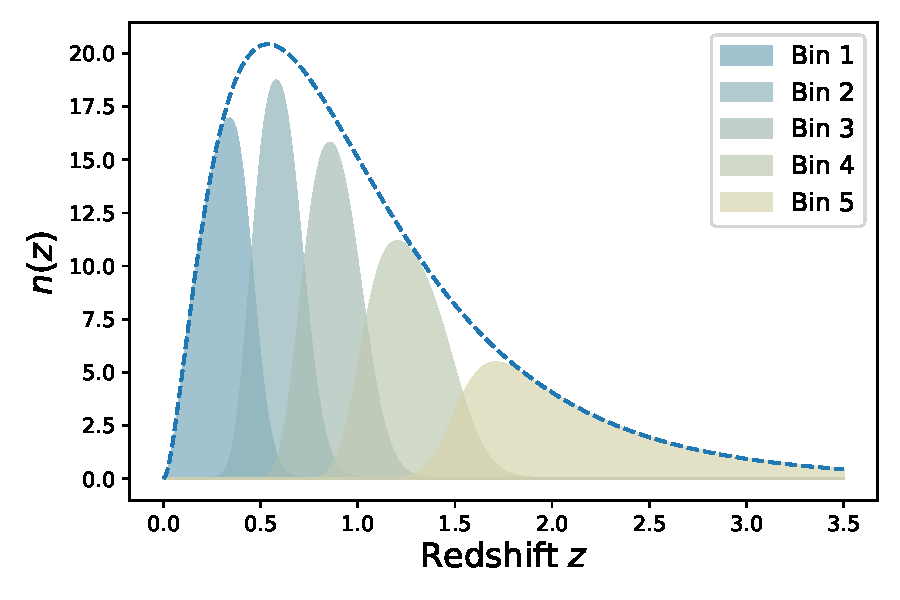
\includegraphics[width=\columnwidth]{figures/redshift_distribution_light.pdf}
    \caption{
     Source sample redshift distributions for each tomographic bin for LSST Y10. The number density on the y-axis is shown in arcmin$^2$.
    }
     \label{fig:redshift_distribution}
\end{figure}
%--------------------------------------------------------------------
%--------------------------------------------------------------------
%--------------------------------------------------------------------
%------------------------------------------------------------------
\section{Experiment}\label{Sec:experiment}
%--------------------------------------------------------------------
%--------------------------------------------------------------------
%--------------------------------------------------------------------
\subsection{Explicit Inference}
%--------------------------------------------------------------------
%--------------------------------------------------------------------
%--------------------------------------------------------------------
\subsubsection{Power spectrum}
%--------------------------------------------------------------------
%--------------------------------------------------------------------
%--------------------------------------------------------------------
Although this is not a full-field approach, we aim to compare the latest to a more standard approach. 
To obtain the probability distribution of the cosmological parameters using a summary-statistics-methods, we focus on the 2-point statistics, specifically, on the angular power spectra $C_{\ell}$.
The correlation between two generic tomographic bins $i$ and $j$ can be expressed as:
\begin{equation}
    \left \langle \kappa^{i}(\ell)\kappa^{j*}(\ell)\right \rangle =(2\pi)^2\delta_D(\ell-\ell')C_{\ell}^{ij},
\end{equation}
We assume a Gaussian likelihood with a cosmology-independent covariance matrix:
\begin{equation}
    \log{\mathcal{L}}(\bm{\theta})=-\frac{1}{2}[\bm{d}-\bm{\mu}(\bm{\theta})]^{T}\bm{C}^{-1}[\bm{d}-\bm{\mu}(\bm{\theta})].
\end{equation}
To compute the expected theoretical predictions $\bm{\mu}(\bm{\theta})$ we use the public library \href{https://github.com/DifferentiableUniverseInitiative/jax_cosmo}{\texttt{jax-cosmo}}. 
 The Covariance matrix $\bm{C}$ of the observables is computed at the fiducial cosmology, shown in \autoref{tab:prior}, using the same theoretical library. In {\texttt{jax-cosmo}}, the Gaussian covariance matrix is defined as:
\begin{equation}
    \text{Cov}(C_{\ell},C_{\ell}')=\frac{1}{f_{sky}(2 \ell+1)}\left(C_{\ell}+\frac{\sigma_{\epsilon}^2}{2n_s}\right)
\end{equation}
where $f_{sky}$ is the fraction of sky observed by the survey, and $n_s$ is the number density of galaxies. 
To obtain the data vector $\bm{d}$, containing the auto- and the cross-power spectra for each tomographic bin, we use the \href{https://lenstools.readthedocs.io/en/latest/lenstool} {\texttt{LensTools}} package \citep{2016A&C....17...73P} on a single noisy simulated map. 
%--------------------------------------------------------------------
%--------------------------------------------------------------------
%--------------------------------------------------------------------
\subsubsection{Full field and HMC}
%--------------------------------------------------------------------
%--------------------------------------------------------------------
%--------------------------------------------------------------------
The following steps outline our methods. We draw cosmological parameters from the priors illustrated in \autoref{tab:prior}. Given values for the cosmological parameters, we generate the log-normal field as described in the previous sections. So, in other words, the simulator becomes the physical model generating a non-linear representation of the convergence map. The measure of the convergence for each pixel and for each bin predicted from the physical model will differ from the ones from real observations due to the noise.  This is taken into account in the likelihood. Specifically, for LSST Y10 the number of galaxies for each pixel should be sufficiently high that for the central limit theorem, we can assume that the observation is characterized by a Gaussian noise $\sigma_n^2=\sigma_e^2/N_s$, with $N_s$ the total number of source galaxies per bin and pixel. Given $\sigma_n^2$ the variance of this Gaussian likelihood, its form in the log form can be expressed as:
\begin{equation}
    \log{\mathcal{L}}(\bm{\theta})=
    \sum_i^{N_{pix}} \sum_{j}^{N_{bins}} \log{P(\kappa^{obs}_{i,j}|\kappa_{i,j},\bm{\theta})}
    =\sum_i^{N_{pix}} \sum_{j}^{N_{bins}}\frac{[\kappa_{i,j}-\kappa^{obs}_{i,j}]^2}{2\sigma_n^2}
\end{equation}
Not relying on any summary statistics, the full-field approach typically results in a high-dimensional problem, requiring more sophisticated statistical techniques. To sample the posterior distribution for $\bm{\theta}$, we use a Hamiltonian Monte Carlo (HMC) algorithm. The HMC algorithm is particularly helpful in high-dimensional spaces where a large number of steps are required to effectively explore the space. It improves the sampling process by using the information contained in the gradients to guide the sampling process. Since the code is implemented in Jax, the gradients are accessible via automatic differentiation. 
%--------------------------------------------------------------------
%--------------------------------------------------------------------
%--------------------------------------------------------------------
\subsection{Implicit Inference}
%--------------------------------------------------------------------
%--------------------------------------------------------------------
%--------------------------------------------------------------------
\subsubsection{Benchmark compression scheme}
To ensure the scalability of density estimation LFI in cases where forward simulations are computationally expensive, it becomes necessary to employ compression techniques that reduce the dimensionality of the data space and extract summary statistics. 
Specifically, we try to find a function $\bm{t}=F(\bm{d})$, where $\bm{t}$ represents low-dimensional summaries of the original data vector $\bm{d}$. The objective is to achieve a compression function $F(\bm{d})$ that maximizes the information while minimizing dimensionality. Previous studies \citep{alsing2018generalized} have demonstrated that, under specific conditions, a compression scheme can be achieved where the dimension of the summaries dim($\bm{t}$) is equal to the dimension of the unknown parameters dim($\bm{\theta}$) without any loss of information at the Fisher level. Multiple approaches exist in an attempt to satisfy this condition. This section aims to provide an overview of the various neural compression-based methods employed in previous works.
%--------------------------------------------------------------------
\paragraph{\textcolor{violet}{Mean Square Error (MSE)}}
%--------------------------------------------------------------------
One of the commonly used techniques for training a Neural Network is by minimizing the $L_2$ norm or Mean Square Error (MSE).
This methods has been widely adopted in various previous studies  \citep{ribli2018improved, lu2022simultaneously, lu2023cosmological}, where the loss function is typically formulated as follows:
\begin{equation}
   \mathcal{L}=\frac{1}{N_{\theta}}(\bm{t}-\bm{\theta})^2.
\end{equation}
Here $N_{\theta}$ represents the number of cosmological parameters, $\bm{t}$ denotes the summary statistics, and $\bm{\theta}$ corresponds to the data vector of the cosmological parameters. 
However, it is important to note that this approach does not guarantee the recovery of maximally informative summary statistics. While this may hold true for fixed fiducial values of the cosmological parameters and assumptions of Gaussianity, its validation to more generic cases need to be proved. Indeed, minimizing the $L_{2}$ norm is equivalent to training the model to estimate the mean of the posterior distribution. We prove this statement in \autoref{Sec:appendix_Mean Square Error}.
%--------------------------------------------------------------------
\paragraph{\textcolor{violet}{Maximum Absolute Error (MAE)}}
%--------------------------------------------------------------------
Another commonly used approach involves minimizing the $L_1$ norm or Mean Absolute Error (MAE). In this approach, the loss function is defined as:
\begin{equation}
    \mathcal{L}=|\bm{t}-\bm{\theta}|
\end{equation}
where $\bm{t}$ represents the summary statistics and $\bm{\theta}$ denotes the cosmological parameters.
In \autoref{Sec:appendix_Maximum Absolute Error}, we demonstrate that minimizing this loss function is equivalent to training the model to estimate the median of the posterior distribution. While extensively employed in various previous studies \citep{2018PhRvD..97j3515G, fluri2018cosmological, ribli2019weak}, similar to the previous consideration for the MSE, it is important to note that the effectiveness of this loss function in extracting sufficient statistics needs to be demonstrated in more generic applications.
%--------------------------------------------------------------------
\paragraph{\textcolor{violet}{Variational Mutual Information Maximization (VMIM)}}
%--------------------------------------------------------------------
The Variational Mutual Information Maximization (VMIM) technique was first introduced for cosmological inference problems by \citet{jeffrey2021likelihood}. This approach aims to maximize the mutual information $I(\bm{t}, \bm {\theta})$ between the cosmological parameters $\bm{\theta}$ and the summary statistics $\bm{t}$.
In the VMIM approach, the loss function is defined as:
\begin{equation}\label{Eq:Loss_vmim}
    \mathcal{L}=- \log{q(\bm{\theta}|\bm{t};\bm{\varphi'})}.
\end{equation}
Here, $q(\bm{\theta}|\bm{t};\bm{\varphi'})$ represents a variational conditional distribution, $\bm{t}$ denotes the summary statistics, $\bm{\theta}$ corresponds to the data vector of the cosmological parameters, and $\bm{\varphi'}$ are the parameters of the Neural Network.
In order to understand the significance of this loss function, it is necessary to start by considering the mathematical definition of mutual information $I(\bm{t}, \bm {\theta})$:
\begin{align}\label{Eq:mutual_information}
    I(\bm{t}, \bm {\theta}) &= D_{KL}(p(\bm {t}, \bm {\theta})||p(\bm {t})p(\bm {\theta})) \\ \nonumber
    &= \int d^n \bm{\theta} d^n \bm{t} p(\bm t, \bm \theta)\log{\left( \frac{ p(\bm {t}, \bm {\theta})}{ p(\bm {t}) p(\bm {\theta})} \right)} \\ \nonumber
    &= \int d^n \bm{\theta} d^n \bm{t} p(\bm t, \bm {\theta})\log{\left( \frac{ p(\bm {\theta} | \bm {t} )}{ p(\bm {\theta})} \right)} \\ \nonumber
        &= \int d^n \bm{\theta} d^n \bm{t} p(\bm t, \bm {\theta})\log{p(\bm {\theta} | \bm {t} )} - \int d^n \bm{\theta}  d^n \bm{t} p(\bm t, \bm {\theta})\log{p(\bm {\theta})} \\ \nonumber
    &= \int d^n \bm{\theta} d^n \bm{t} p(\bm t, \bm {\theta})\log{p(\bm {\theta} | \bm {t} )} - \int d^n \bm{\theta} p(\bm {\theta})\log{p(\bm {\theta})} \\ \nonumber
    &= \mathbb{E}_{p(\bm {t}, \bm {\theta})} [\log{p(\bm {\theta} | \bm {t} )}]- \mathbb{E}_{p(\bm {\theta})} [\log{p(\bm {\theta})}] \\ \nonumber
    &= \mathbb{E}_{p(\bm {t}, \bm {\theta})} [\log{p(\bm {\theta} | \bm {t} )}]- H(\bm {\theta});
\end{align}

in the above equation, $D_{KL}$ is the Kullback-Leibler divergence \citep{kullback1951information}, $p(\bm {t}, \bm {\theta})$ is the joint probability distribution of summary statistics and cosmological parameters, and $H(\bm {\theta})$ represents the \textit{entropy} of the distribution of cosmological parameters.  
Essentially, mutual information measures the amount of information contained in the summary statistics $\bm t$ about the cosmological parameters $\bm \theta$. The summary statistics $\bm{t}$ are extracted from the original high-dimensional data vector $\bm{d}$ using $\bm{t}=F_{\bm {\varphi}}(\bm{d})$.
The goal is to find the parameters $\bm {\varphi}$ that maximize the mutual information between the summary and cosmological parameters:
\begin{equation}
   \bm {\varphi}^*= \operatorname*{argmax}_{\bm {\varphi}} I(F_{\bm {\varphi}}(\bm{d}), \bm {\theta}).
\end{equation}
However, the mutual information expressed in \autoref{Eq:mutual_information} is not tractable. To overcome this limitation, various approaches have been developed that rely on tractable bounds, enabling the training of deep neural networks to optimize the mutual information. In this study, we adopt the same strategy used by \citet{jeffrey2021likelihood}, which involves using the variational lower bound \citep{barber2003information}:
\begin{equation}\label{Eq:variational_lower_bound}
    I(\bm{t}, \bm{\theta}) \ge \mathbb{E}_{p(\bm {t}, \bm {\theta})} [\log{q(\bm {\theta} |\bm{t} ; \bm{\varphi}')}]- H(\bm {\theta}).
\end{equation}
Here, the variational conditional distribution $\log{q(\bm {\theta} |\bm{t}; \bm{\varphi}')}$ is introduced to approximate the true posterior distribution $p(\bm{\theta}|\bm {t})$. 
As the entropy of the cosmological parameters remains constant for a fixed training set, the optimization problem based on the lower bound in \autoref{Eq:variational_lower_bound} can be formulated as:
\begin{equation}
    \operatorname*{argmax}_{\bm {\varphi}, \bm {\varphi}'}\mathbb{E}_{p(\bm {d}, \bm {\theta})} [\log{q(\bm {\theta} |F_{\bm {\varphi}}(\bm {d}) ; \bm{\varphi}')}], 
\end{equation}
yielding \autoref{Eq:Loss_vmim}.
%--------------------------------------------------------------------
\paragraph{\textcolor{violet}{Gaussian Negative Log-Likelihood (GNLL)}}
%--------------------------------------------------------------------
\FL{Recognizing that the uncertainty on different cosmological parameters will vary, a third
class of inverse variance weighted MSE was proposed in \cite{fluri2018cosmological} with the idea of
ensuring that each parameter contributes fairly to the overall loss by taking into account its uncertainty. The loss function typically takes the following form:
\begin{equation}
    \mathcal{L} = \frac{1}{2} \log(|\Sigma|) + \frac{1}{2}(t - \theta)^t \Sigma^{-1} (t - \theta) 
\end{equation}
where $t$ is the summary statistics and $\Sigma$ is the covariance matrix of representing the uncertainty on the cosmological parameters $\theta$. Both $t$ and $\Sigma$ can be outputs of the compression network, i.e. $f_\theta(x)=(t, \Sigma)$.

One recognizes here the expression of a Gaussian probability function, and this expression can thus be straightforwardly related to the VMIM case by simply assuming a Gaussian distribution as the variational approximation for the posterior $q(\theta | x) = \mathcal{N}(\theta; t, \Sigma)$.

This means that this loss function is actually sub-optimal for two reasons:
\begin{itemize}
    \item The summary extracted by the neural network $t$ is, similarly to the MSE case only an estimate of the mean of 
    the posterior distribution, which is not guaranteed to be sufficient.
    \item Because of the Gaussian variational assumption, the variational posterior can potentially be biased with respect to the true posterior, and thus the mean of this Gaussian approximation may be biased with respect to the true posterior mean.
\end{itemize}
 A simple MSE would thus seem to be preferable.
}
%--------------------------------------------------------------------
\paragraph{\textcolor{violet}
{Information Maximising Neural Networks (IMNNs)}}. \LM{TODO: condensed introduction; emphasize learning compression at single point; network learns score function which generalises smoothly away from fiducial \cite{Makinen_2021, Makinen_2022, Charnock_2018}, Wandelt (in prep.) 
}

%--------------------------------------------------------------------

%--------------------------------------------------------------------
%--------------------------------------------------------------------
%--------------------------------------------------------------------
\subsubsection{Inference strategy}
%--------------------------------------------------------------------
%--------------------------------------------------------------------
By comparing the posteriors $p(\theta| t)$ obtained with different compression strategies, we can assess the sensitivity of the results to the choice of statistics. In particular, the more informative the summary statistics, the “closer” the posterior $p(\theta | t)$ is to the true posterior $p(\theta | x)$. In this section, we describe how we approximate the posterior distribution for each summary statistic t, enable us to use it as a fair benchmark for comparison (we describe the performance metric in section ??).\\
Since the likelihood $p(t|\theta)$ is intractable, we propose to do Neural Posterior Estimation \citep{npe1, npe2, npe3}, a Simulation-Based Inference (SBI) strategy that aims to directly approximate, from simulations, the posterior distribution 

\begin{equation}
    p(\theta | t) \propto \int p(t | \theta, z) p(z|\theta) p(\theta) dz\,.
\end{equation}

Usually, NPE algorithm approximates the posterior distribution through the use of conditional Normalizing Flows $p_{\varphi} (\theta | t)$ \citep{nf1, nf2}. This is achieved by minimizing the negative log probability: 

\begin{equation}
    \mathbb{E}_{p(\theta, t)} \left[ - \log p_{\varphi} (\theta | t)  \right].
    \label{eq:nll}
\end{equation}

Finally, the target posterior $p(\theta | t = t_0)$ is approximated by $p_{\varphi}(\theta | t = t_0)$ where $t_0 = t(x_0)$ with $x_0$ the observed convergence map.

For each summary statistic, we approximate it posterior distribution using the same NF architecture, namely a RealNVP \citep{realnvp} with 4 coupling layers, shift and scale parameters are learned using a neural network with 2 layers of 128 neurons, activation functions are $silu$ \citep{silu}. And, for each summary statistic, the prior $p(\theta)$ used in the inference process remains the same.
%--------------------------------------------------------------------
%--------------------------------------------------------------------
\subsection{Result estimators}
%--------------------------------------------------------------------
%--------------------------------------------------------------------
To evaluate the results obtained from different approaches, we use two commonly employed estimators found in the literature. Their definitions are provided in the following sections.
%--------------------------------------------------------------------
\subsubsection{Figure of Merit (FoM)}
To quantify the constraining power of each inference strategy, we first employ the Figure of Merit (FoM), defined as follows:
\begin{equation}\label{Eq:Figure_of_merit}
    \text{FoM}_{\alpha \beta}=\sqrt{\text{det}(\Tilde{F}_{\alpha \beta})}.
\end{equation}
Here, $\alpha$ and $\beta$ represent a pair of cosmological parameters, and $\Tilde{F}_{\alpha \beta}$ refers to the marginalized Fisher matrix. We calculate $\Tilde{F}_{\alpha \beta}$ as the inverse of the parameter space covariance matrix $C_{\alpha \beta}$, which is estimated from the HMC chains and from the Normalizing flow sampling. 
Under the assumption of a Gaussian covariance, the FoM defined in \autoref{Eq:Figure_of_merit} is proportional to the inverse of the $2-\sigma$ contours in the 2-dimensional marginalised parameter space of the $\alpha$ and $\beta$ pair.
\subsubsection{Kullback-Leibler divergence}
%--------------------------------------------------------------------
\begin{center}
\begin{table*}
\begin{tabular}{ |p{3.5cm}|p{2cm}|p{3cm}|p{2.5cm}|p{4cm}|  }
 \hline
Reference & \makecell{Architecture\\ compressor}  & \makecell{Loss function} & \makecell{Inference \\ strategy} & \makecell{Output compressor}   \\
 \hline
            \citet{2018PhRvD..97j3515G} & \makecell{CNN} & \makecell{MAE} &  \makecell{Likelihood \\ analysis} &\makecell{$\sigma_8, \Omega_m$}  \\
 \hline
            \citet{fluri2018cosmological} & \makecell{CNN} & \makecell{MAE} & \makecell{Likelihood \\ analysis} &  \makecell{$\log{(\sigma_{\Omega_m}^2)},\log{(\sigma_{\sigma_8}^2)}$,
             \\
            $\tanh^{-1}{(\text{Corr}(\sigma_8,\Omega_m))}$,
             \\
            $\sigma_8,\Omega_m$} 
\\
\hline     
\rowcolor{lightgray}
            \citet{fluri2019cosmological} & \makecell{CNN} & \makecell{GNLL} & \makecell{Likelihood \\ analysis} & \makecell{$\sigma_8, \Omega_m, A_{IA}/10, L$  \\ with  $L:\Sigma^{-1}=LL^{T}$}
\\
\hline            
            \citet{ribli2018improved} & \makecell{CNN} & \makecell{MSE}  &\makecell{RMSE for \\ evaluation}  & \makecell{$\sigma_8, \Omega_m$}   
\\
\hline            
            \citet{ribli2019weak} & \makecell{CNN} & \makecell{MAE} & \makecell{Likelihood \\ analysis} & \makecell{$\sigma_8, \Omega_m$}   
\\            
\hline             
            \citet{PhysRevD.102.123506} & \makecell{CNN} & \makecell{MAE} & \makecell{Likelihood \\ analysis} & \makecell{$\sigma_8, \Omega_m$}   
\\
\hline 
\rowcolor{lightgray}
            \citet{jeffrey2021likelihood} & \makecell{\makecell{CNN} \\\makecell{CNN}+NF} & 
            \makecell{MSE \\ VMIM}
            & \makecell{PyDelfi} & \makecell{$\varphi: F_{\varphi}(\bm{d})=\bm{\theta}$ \\ with $\bm{\theta}=\Omega_m, \sigma_8$}    
\\            
\hline             
            \citet{fluri2021cosmological} & \makecell{GCNN} & \makecell{IMNN} & \makecell{GPABC} &  
\\
\hline      
\rowcolor{lightgray}

            \citet{fluri2022full} & \makecell{GCNN} & \makecell{IMNN} & \makecell{GPABC} &  
\\            
\hline 
            \citet{lu2022simultaneously} & \makecell{CNN} & \makecell{MSE} & \makecell{Likelihood \\ analysis}  & \makecell{$\Omega_m,S_8, A_{IA}/10,$ \\ rescaled \\ baryonic parameters \\ $(M_c,M_{1,0}, \eta, \beta)$}   
\\           
\hline 
            \citet{kacprzak2022deeplss} & \makecell{CNN} & \makecell{GNLL}  & \makecell{Likelihood \\ analysis}  & \makecell{WL: $\Sigma, \Omega_m, \sigma_8, A_{IA}, \eta_{IA}$ \\  GC:$\Sigma, \Omega_m, \sigma_8, b_g, r_g,\eta_{b_{g}}$ }
          
\\
\hline 
\rowcolor{lightgray}
            \citet{lu2023cosmological} & \makecell{CNN} & \makecell{MSE} & \makecell{Likelihood \\ analysis}  & \makecell{$\Omega_m,S_8,A_{IA}/10,$\\ rescaled baryonic \\ parameters: $M_c,M_{1,0}, \eta, \beta$} 
\end{tabular}
\label{tab:biblio_survey}
\end{table*}
\end{center}
%--------------------------------------------------------------------
\section{Results}\label{Sec:results}
%--------------------------------------------------------------------
We present the results of the constraints on the full $\Lambda$CDM parameter space expected for a survey like LSST-Y10. The forecasted results are obtained using the simulation procedure outlined in and the parameter inference strategy described in .
We begin by comparing the outcomes of three different inference procedures: Explicit 2-point statistics, Explicit full-field statistics, and Implicit statistics using CNN summaries. Subsequently, we analyze the impact of the different compression strategies on the final cosmological constraints.
%--------------------------------------------------------------------
\subsection{Power spectrum and full-field statistics}
%--------------------------------------------------------------------
We now compare the constraining power of the three different approaches described in \autoref{Sec:experiment}: the standard-two point statistics and two map-based approaches, the explicit inference using an HMC and the implicit inference using the Normalizing Flow as an estimator. 
As outlined before, our interest is to prove that the two map-based approaches lead to very comparable posterior distributions. We present the constraints in the full $\Lambda$CDM parameter space in \autoref{fig:contours_posterior_imp_ex_ps}. The contours obtained by the angular $C_{\ell}$ analysis are plotted in blue, the ones for the HMC in yellow, and those for the Normalizing Flow in violet. Confirming previous work, we find the two-point statistics are suboptimal in constraining $\Omega_c$, $\sigma_8$, and $w_0$. $h$, $\Omega_b$, and $n_s$ result prior dominated and hence are constrained by none of the three approaches. 
 We quantify the results by computing the Figure of Merit as described in \autoref{Eq:Figure_of_merit}. The results are presented in \autoref{tab:f_o_m}. 
A further investigation is represented by 
-show the results for the KL divergence 
-present a comparison with other works. 
%--------------------------------------------------------------------
% ############# PLOT CONTOURS HMC-SBI-PS  #############
%--------------------------------------------------------------------
\begin{figure*}
    \centering
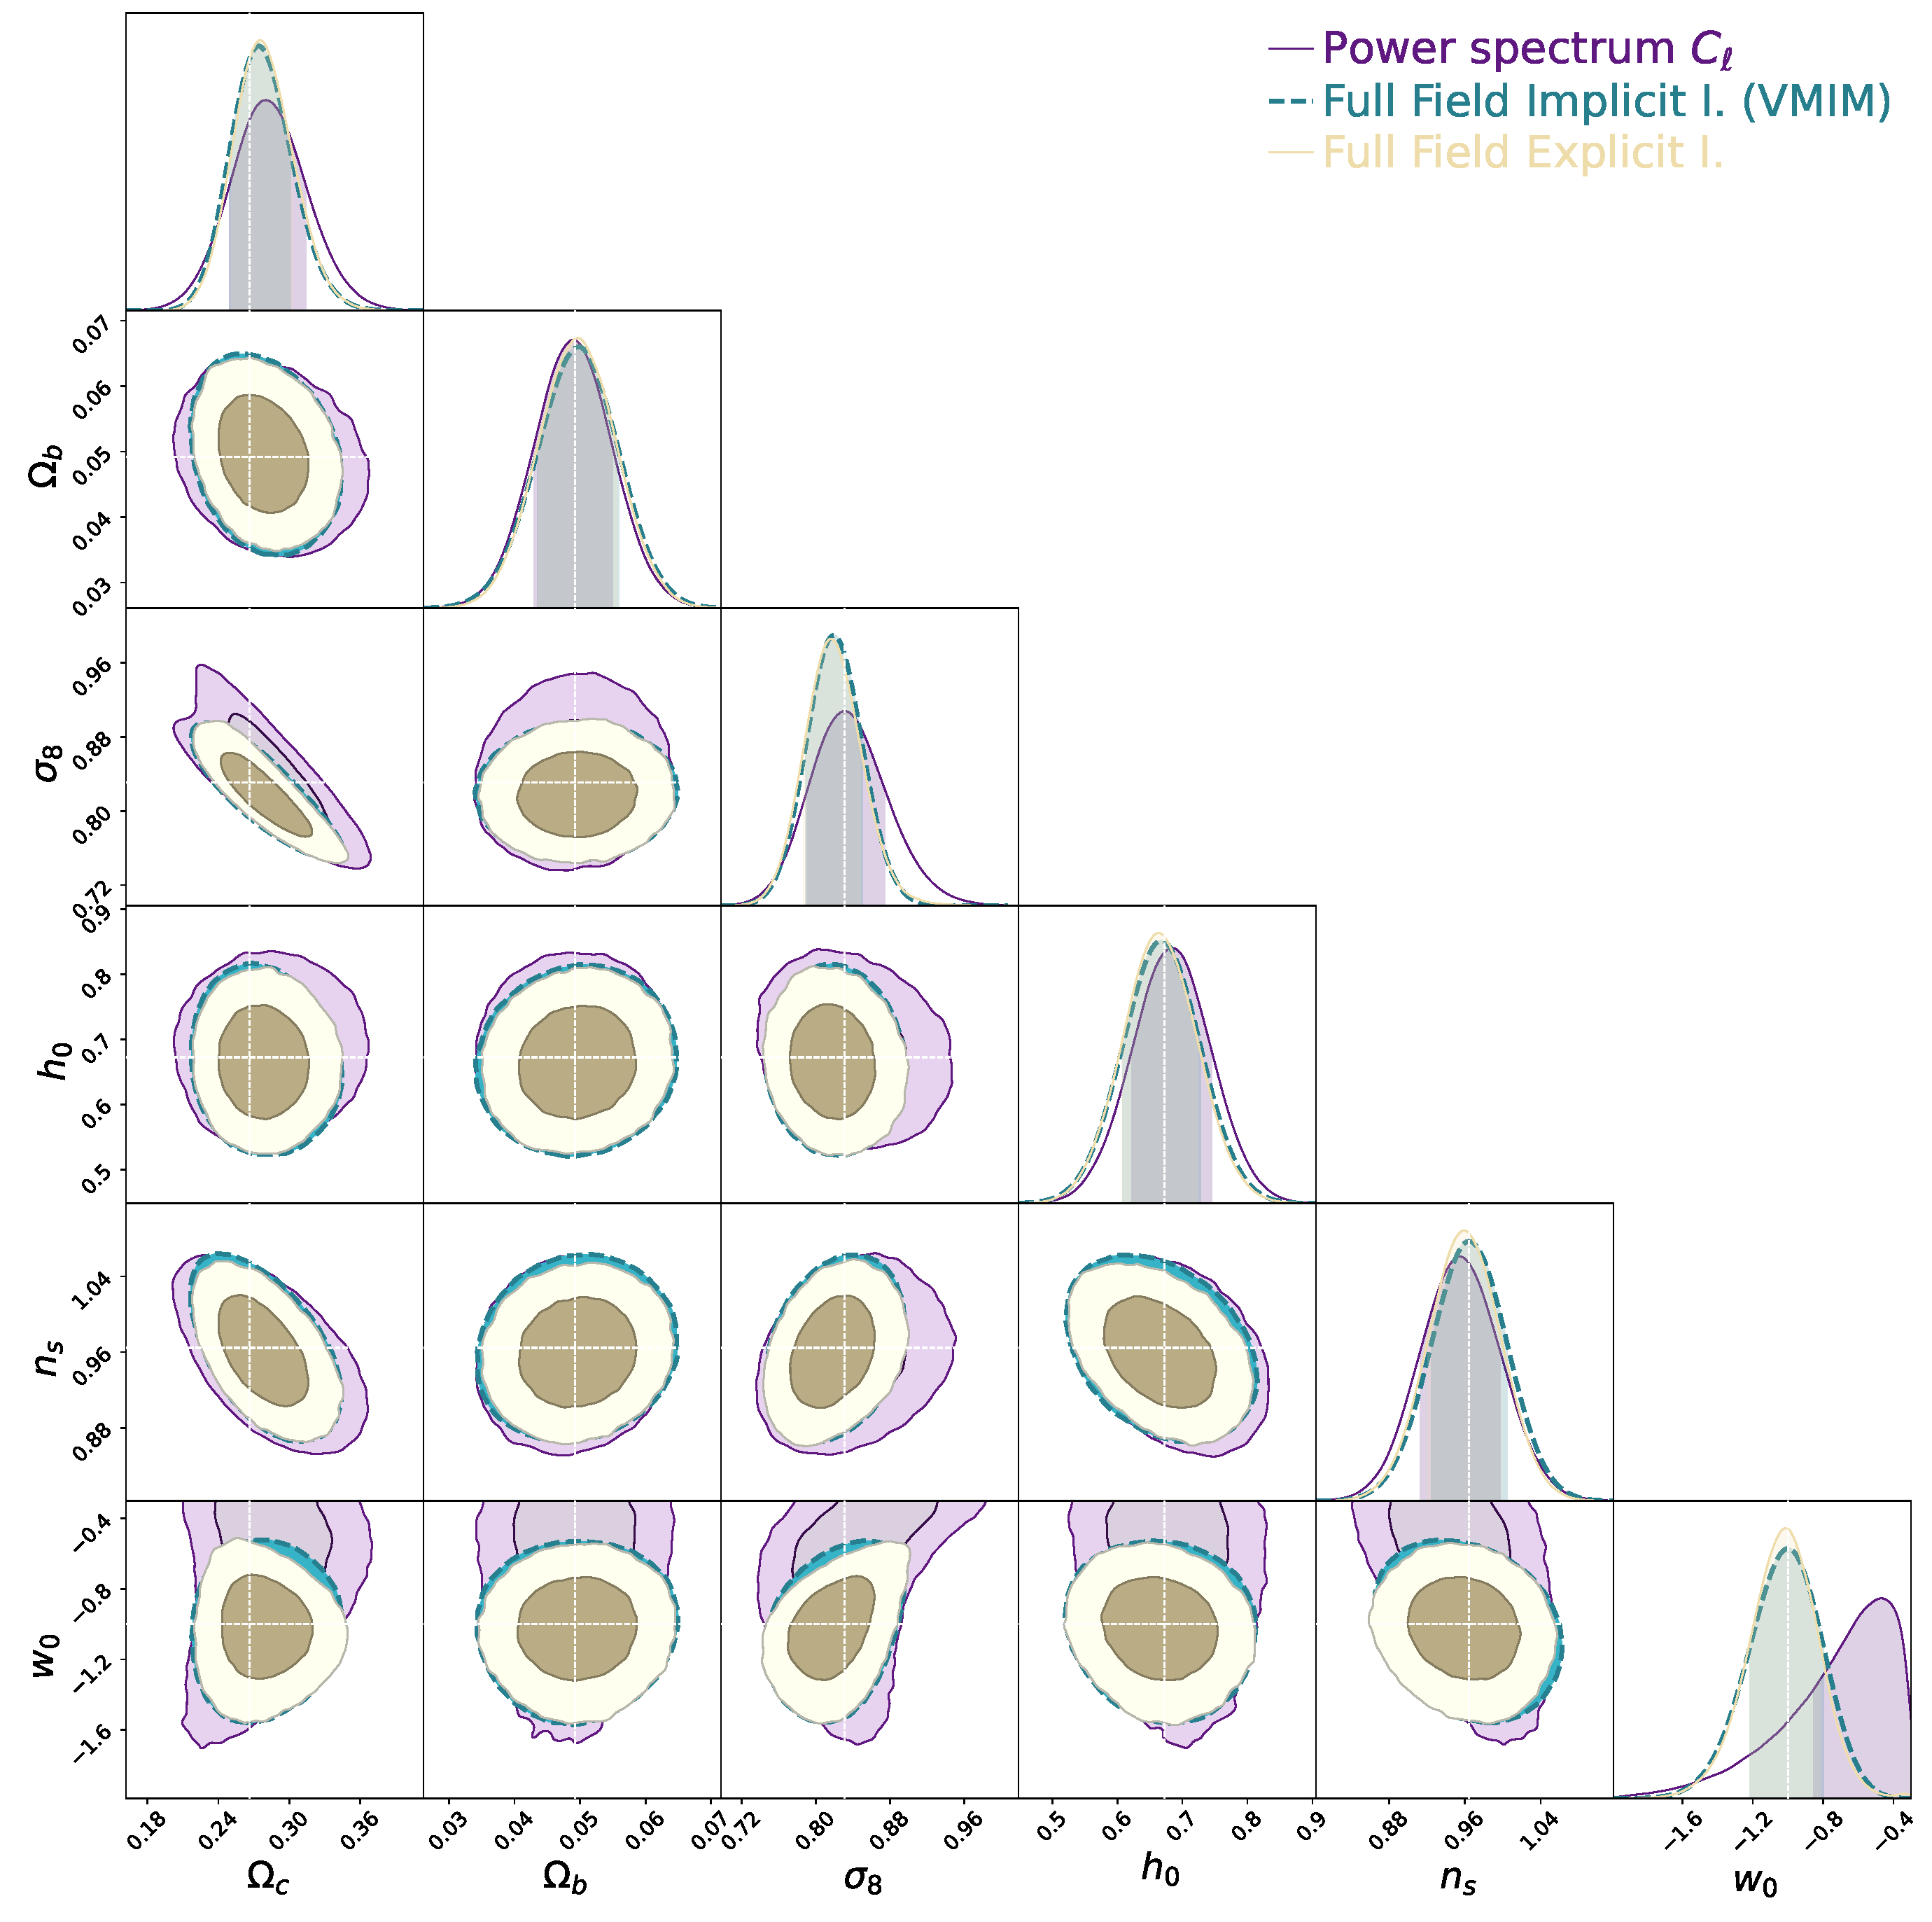
\includegraphics[width=\textwidth]{figures/contours_posterior_imp_ex_ps.pdf}
    \caption{
Constraints on the $\Lambda$CDM parameter space as found in the LSST Y10 survey setup. The constraints are obtained by applying the $C_{\ell}$ (light blue contours), the full field explicit inference (yellow contours), and the full field implicit inference strategy (violet contours), described in \autoref{Sec:experiment}.
The contours show the $68\%$ and the $95\%$  confidence regions. The dashed white lines define the true parameter values.}
\label{fig:contours_posterior_imp_ex_ps}
\end{figure*}
%--------------------------------------------------------------------
% ############# FIGURE OF MERIT TABLE  #############
%--------------------------------------------------------------------
\begin{center}
\begin{table*}
\caption{ Values of the Figure of Merit (FoM) as defined in \autoref{Eq:Figure_of_merit} for different inference strategies: the convergence power spectrum $C_{\ell}$, the HMC, the CNN map compressed statistics with the MSE, the VMIM, the MAE and the GNLL loss functions. The values of the figure of merit are inversely proportional to the area of the contours, larger the FoM, higher the constraining power.}
\begin{tabular}{lcccccc} 
 \hline
    FoM & $C_{\ell}$ & Full Field (HMC)&  VMIM & MSE & MAE & GNLL   \\
  \hline\hline
 $\Omega_c-  \Omega_b$ & 5315 & 6951 & 6591 & 5651 & 5909\\
 $\Omega_c-  \sigma_8$ & 1222 & 2520 & 2526 & 2043 & 2316\\
 $\Omega_c-  h_0$      & 516  & 698  & 675  & 601  & 618\\
 $\Omega_c-  n_s$      & 898  & 1243 & 1184 & 964  & 1030\\
 $\Omega_c-  w_0$      & 100  & 198  & 190  & 152  & 162\\
 $\Omega_b-  \sigma_8$ & 3997 & 5472 & 5514 & 5066 & 5398\\
 $\Omega_b-  w_0$      & 523  & 846  & 791  & 736  & 771\\
 $\sigma_8-  h_0$      & 402  & 566  & 577  & 544  & 571\\
 $\sigma_8-  n_s$      & 583  & 889  & 891  & 787  & 854\\ 
 $\sigma_8-  w_0$      & 77   & 176  & 171  & 139  & 149\\
 $h_0-       w_0$      & 52   & 88   & 83   & 80   & 82\\
 $n_s-       w_0$      & 80   & 133  & 126  & 112  & 119 \\
     \hline
\end{tabular}
\label{tab:f_o_m}
\end{table*}
\end{center}
%--------------------------------------------------------------------
%  ############# SUMMARY TABLE  #############
%--------------------------------------------------------------------
\begin{table*}
  \begin{tabular}{|l|l|l|l|l|l|l|l|l|}
    \hline
    \multirow{2}{*}{} &
      \multicolumn{2}{c|}{VMIM} &
      \multicolumn{2}{c|}{MSE} &
      \multicolumn{2}{c|}{MAE} &
      \multicolumn{2}{c|}{GNLL} \\
    & Mean & $\sigma$ & Mean & $\sigma$ & Mean & $\sigma$  & Mean & $\sigma$ \\
    \hline
    $\Omega_c$ & 0.2742 & 0.026 & 0.2830 & 0.030 & 0.2793 & 0.029  & 2.1\% & 2.1\%\\
    \hline
    $\Omega_b$ & 0.0499 & 0.006 & 0.0492 & 0.006 &  0.0501 & 0.006 & 2.1\% & 2.1\% \\
    \hline
    $\sigma_8$ & 0.819 & 0.03 &0.808 & 0.03 &  0.808 &0.03 & 2.1\% & 2.1\% \\
    \hline
    $w_0$      &-0.998 & 0.2 &-1.13 & 0.2 & -1.16& 0.2  & 2.1\% & 2.1\% \\
    \hline
    $h_0$      & 0.6658 & 0.058 &0.6620 & 0.057 & 0.6640 & 0.057&  2.1\% & 2.1\% \\
    \hline
    $n_s$      & 0.9635 & 0.04 & 0.9559 & 0.04 & 0.9547 & 0.04  & 2.1\% & 2.1\% \\
    \hline
  \end{tabular}
\end{table*}
%--------------------------------------------------------------------
%--------------------------------------------------------------------
\section{Conclusions}\label{Sec:conclusion}
%--------------------------------------------------------------------
%--------------------------------------------------------------------
\begin{acknowledgements}
This work was granted access to the HPC/AI resources of IDRIS under the allocation 2022-AD011013922 made by GENCI.
\end{acknowledgements}
%--------------------------------------------------------------------
%              #########    START BIBLIO   #########
%--------------------------------------------------------------------
\bibliographystyle{aa} % style aa.bst
\bibliography{paper/biblio} 
%--------------------------------------------------------------------
%              #########    START APPENDIX   #########
%--------------------------------------------------------------------
\begin{appendix}
\section{Mean Square Error (MSE)}\label{Sec:appendix_Mean Square Error}
In this section, we demonstrate that minimizing the $L_2$ norm is equivalent to training the model to estimate the mean of the posterior distribution, namely:
\begin{equation}\label{Eq:mean_mse}
\left \langle \bm {\theta} \right \rangle_{p(\bm {\theta}|\bm{d})}=\operatorname*{argmin}_{\mathcal{F}(\bm{d})}\mathbb{E}_{p(\bm {\theta}|\bm {d})}[\left\Vert \bm {\theta}-\mathcal{F}(\bm{d})
 \right \Vert_{2}^{2}].
\end{equation}
To demonstrate \autoref{Eq:mean_mse}, we need to minimize the expected value of the $L_2$ norm with respect to $\mathcal{F}(\bm{d})$. Let us consider its derivative:
\begin{align}\label{Eq:moment_1}
   & \frac{\partial}{\partial \mathcal{F}(\bm{d}) }  \mathbb{E}_{p(\bm {\theta}|\bm{d}))}[(\bm {\theta}-\mathcal{F}(\bm{d}))^2] =  \\
    &
    \frac{\partial}{\partial \mathcal{F}(\bm{d}) }  \mathbb{E}_{p(\bm {\theta}|\bm {d})}[\bm {\theta}^2+\mathcal{F}(\bm{d})^2-2\bm {\theta}\mathcal{F}(\bm{d})] = \nonumber \\
    &
    \frac{\partial}{\partial \mathcal{F}(\bm{d}) }  [
    \mathbb{E}_{p(\bm {\theta}|\bm {d})}[\bm {\theta}^2]+\mathcal{F}(\bm{d})^2-2\mathcal{F}(\bm{d})\mathbb{E}_{p(\bm {\theta}|\bm {d})}[\bm {\theta}]]= \nonumber \\
    &2\mathcal{F}(\bm{d})-2 \mathbb{E}_{p(\bm {\theta}|\bm {d})}[\bm {\theta}]. \nonumber
\end{align}
Setting it equal to zero, we obtain the critical value:
\begin{equation}
    \mathcal{F}(\bm{d})= \mathbb{E}_{p(\bm {\theta}|\bm {d})}[\bm {\theta}]. 
\end{equation}
Considering the second-order derivative:
\begin{equation}\label{Eq:minimum_mean}
   \frac{\partial^2}{\partial^2 \mathcal{F}(\bm{d})}  \mathbb{E}_{p(\bm {\theta}|\bm {d})}[(\bm {\theta}-\mathcal{F}(\bm{d}))^2]=2, 
\end{equation}
we can assert that the critical value $\mathcal{F(\bm(\theta))}$ is also a minimum. 
Since 
\begin{equation}
    \mathbb{E}_{p(\bm {\theta}|\bm {d})}[\bm {\theta}|\bm{d}]= \left \langle \bm {\theta} \right \rangle_{p(\bm {\theta}|\bm{d})}
\end{equation}
it follows from \autoref{Eq:minimum_mean} the \autoref{Eq:mean_mse}.
%--------------------------------------------------------------------
\section{Maximum Absolute Error (MAE)}\label{Sec:appendix_Maximum Absolute Error}
In this section, we demonstrate that minimizing the $L_2$ norm is equivalent to training the model to estimate the median of the posterior distribution.
By definition, the median of a probability density function $p(x)$ is a real number $m$ that satisfies:
\begin{equation}\label{Eq:definition_median}
\int_{\infty}^{m} p(x)dx=\int_{m}^{\infty}p(x)dx=\frac{1}{2}.
\end{equation}. 
The expectation value of the mean absolute error is defined as:
\begin{equation}
    \mathbb{E}[|x-m|]= \int_{\infty}^{\infty}p(x)|x-m|dx  
\end{equation}
which can be decomposed as
\begin{equation}
        \int_{\infty}^{m}p(x)|x-m|dx +\int_{m}^{\infty}p(x)|x-m|dx .
\end{equation}
To minimize this function with respect to $m$, we need to compute its derivative:
\begin{equation}\label{Eq:absolute_median}
    \frac{d\mathbb{E}[|x-m|]}{dm}=
    \frac{d}{dm}\int_{\infty}^{m}p(x)|x-m|dx +\frac{d}{dm}\int_{m}^{\infty}p(x)|x-m|dx. 
\end{equation}
Considering that $|x-m|=(x-m)$ for $m\le x$ and $|x-m|=(m-x)$ $m\ge x$, 
we can write \autoref{Eq:absolute_median} as:
\begin{equation}
    \frac{d\mathbb{E}[|x-m|]}{dm}=
    \frac{d}{dm}\int_{\infty}^{m}p(x)(m-x)dx +\frac{d}{dm}\int_{m}^{\infty}p(x)(x-m)dx .
\end{equation}
Using the Leibniz integral rule, we get:
\begin{align}
    &\frac{d\mathbb{E}[|x-m|]}{dm}= \\
    &
    p(x)(m-m)\frac{dm}{dm}+\int_{\infty}^{m}\frac{\partial}{\partial m}[p(x)(m-x)]dx + \nonumber \\
    & - p(x)(m-m)\frac{dm}{dm}+\int_{m}^{\infty}\frac{\partial}{\partial m}[p(x)(m-x)]dx \nonumber .
\end{align}
Setting the derivative to zero, we obtain:
\begin{equation}
    \frac{d\mathbb{E}[|x-m|]}{dm}= \int_{\infty}^{m} p(x)dx-\int_{m}^{\infty}p(x)dx =0.
\end{equation}
Thus,
\begin{equation}
\int_{\infty}^{m} p(x)dx=\int_{m}^{\infty}p(x)dx .
\end{equation}
Considering that
\begin{equation}
\int_{\infty}^{m} p(x)dx+\int_{m}^{\infty}p(x)dx=1,
\end{equation}
we obtain \autoref{Eq:definition_median}.
% \begin{equation}
% \int_{\infty}^{m} p(x)dx=\int_{m}^{\infty}p(x)dx=\frac{1}{2}.
% \end{equation}
%--------------------------------------------------------------------
%              #########    END APPENDIX   #########
%--------------------------------------------------------------------
\end{appendix}
\end{document}